\section{Electron-Phonon Interactions}
We discussed tight-binding electrons which lead to bands, and lattice vibrations which lead to phonons - but both happen at the same time, so we now ask how do these two interact/intertwine?

Despite a fairly simple Hamiltonian that describes this, it's a surprisingly difficult problem, with unsolved questions remaining to this day.

\subsection{Deriving the Electron-Phonon Interaction Hamiltonian}
We proceed by considering electrons moving in the ionic potential, but we will not assume the ions are frozen in a perfectly periodic formation. We write:
\begin{equation}
    H_1 = \sum_{\v{k}, \v{k}', l}\bra{\v{k}}U_0(\v{r} - \v{R}_l - \gv{\mu}_l)\ket{\v{k}'}c^\dag_{\v{k}}c_{\v{k}'}
\end{equation}
where $U_0$ is a single-ion potential, $\v{R}_l$ is the ion equilibrium position, and $\gv{\mu}_l$ the ion displacement.

As usual, we work in a basis where $\ket{\v{k}} \cong \frac{1}{\sqrt{V}}e^{i\v{k} \cdot \v{r}}$. So we calculate the matrix element, which amounts to fourier transforming the potential of these ions. What we get out is;
\begin{equation}
    H_1 = \sum_{\v{k}, \v{k}', l} e^{i(\v{k}' - \v{k}) \cdot (\v{R}_l + \gv{\mu}_l)}V_{\v{k} - \v{k}'}c^\dag_{\v{k}}c_{\v{k}'}
\end{equation}
Here, $V_{\v{k}}$ is the FT of $U_0(\v{r})$. We will now proceed to make the assumption that $\abs{\gv{\mu}_l} \ll a$ and expand:
\begin{equation}
    e^{i(\v{k}' - \v{k})\cdot\gv{\mu}_l} \approx 1 + i(\v{k}' - \v{k})\gv{\mu}_l = 1 + \frac{i}{\sqrt{N}}(\v{k}' - \v{k})\sum_q e^{i\v{q} \cdot \v{R}_l}\gv{\mu}_q
\end{equation}
We now substitute this back into the equation. The leading term (1) is just the Bloch Hamiltonian:
\begin{equation}
    H_{\text{Bloch}} = \sum_{\v{k}, \v{k}'}\left(\sum_l e^{i(\v{k} - \v{k}')\cdot \v{R}_l}\right)V_{\v{k} - \v{k}'}c^\dag_{\v{k}}c_{\v{k}'} = N\sum_{k, G}V_{\v{G}}c^\dag_{\v{k} + \v{G}}c_{\v{k}}
\end{equation}
this we already studied. Going to the next term, we get electron-phonon interaction:
\begin{equation}
    H_{e-p} = \frac{i}{\sqrt{N}}\sum_{\v{k}, \v{k}'}(\v{k}' - \v{k})\gv{\mu}_{\v{k} - \v{k}'}V_{\v{k} - \v{k}'}c^\dag_{\v{k}}c_{\v{k}'}
\end{equation}
where we again have carried out the sum over lattice indices $l$. Now, let us express $\gv{\mu}_{\v{q}}$ in terms of phonon operators:
\begin{equation}
    H_{e-p} = i\sum_{\v{k}, \v{k}', s}\left(\frac{N\hbar}{2M\omega_{\v{k} - \v{k}', s}}\right)^{1/2}(\v{k}' - \v{k})\cdot \v{s}V_{\v{k} - \v{k}'}(a^\dag_{\v{k}' - \v{k}, s} + a_{\v{k} - \v{k}', s})c^\dag_{\v{k}}c_{\v{k}'}
\end{equation}
Looking at the creation/annihilation operators, we can see that an electron with momentum $\v{k}'$ gets destroyed and a new one with momentum $\v{k}$ is created. In the process, a phonon with that difference is either emitted or created. Diagramatically:

\begin{figure}[htbp]
    \centering
    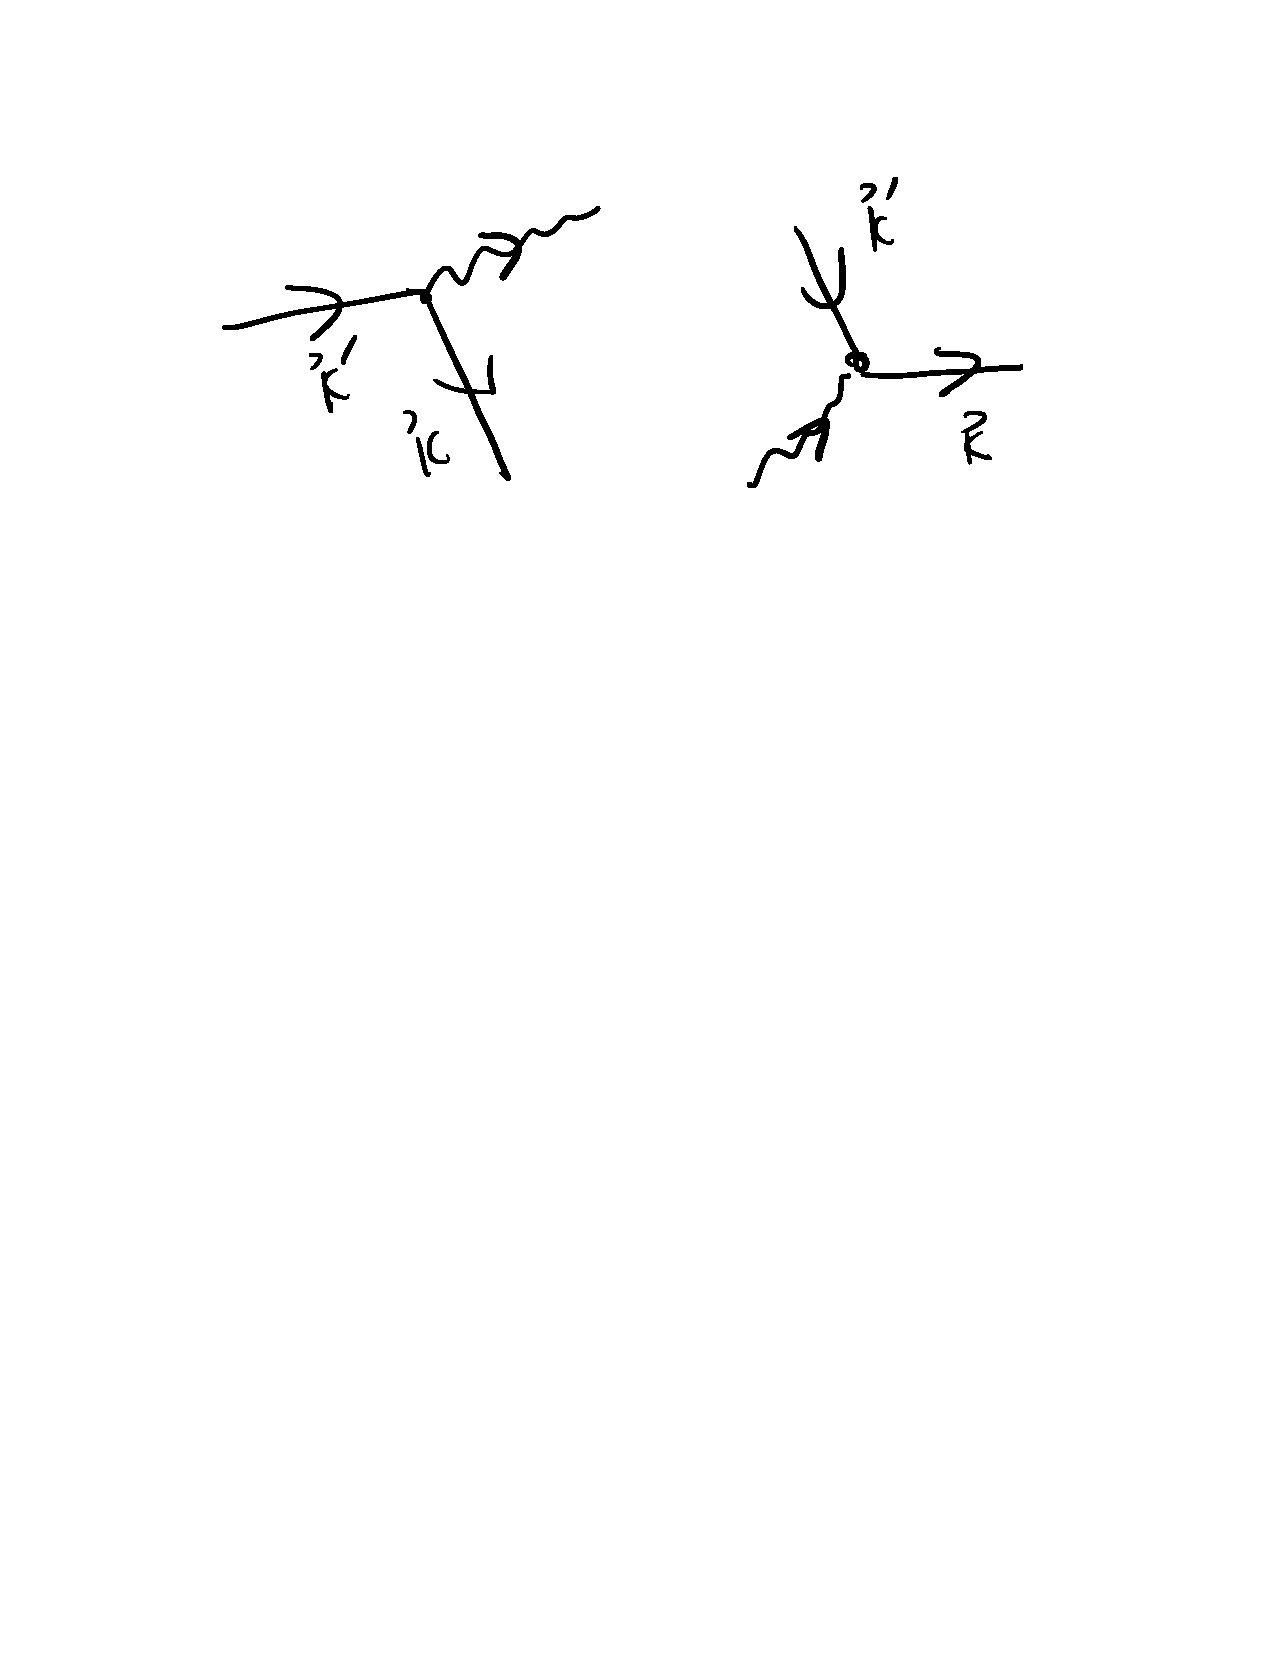
\includegraphics[scale=0.5]{Images/fig-elphfeynman.pdf}
    \caption{Feynman Diagrams for the processes in $H_{e-p}$.}
    \label{fig-elphfeynman}
\end{figure}

Also, look at $(\v{k}' - \v{k})\cdot \v{s}$; this means that only longitudinal phonons are important. In a generic solid, one cannot classify longitudinal/transverse phonons, but let us assume a sufficient amount of isotropy in the solid such that this is possible.

In the following, we make two assumptions:
\begin{enumerate}[(i)]
    \item We only have longitudinal phonons.
    \item Neglect the effect of $H_{\text{Bloch}}$ - study el-ph interactions in the limit of free-electrons.
\end{enumerate}
We therefore have the full Hamiltonian:
\begin{equation}
    H = \sum_{\v{k}}\e_\v{k}c^\dag_\v{k}c_\v{k} + \sum_{\v{q}}\omega_{\v{q}}a^\dag_{\v{q}}a_{\v{q}} + \sum_{\v{k}, \v{q}} M_{\v{q}}(a^\dag_{-\v{q}} + a_{\v{q}})c^\dag_{\v{k} + \v{q}}c_{\v{k}}
\end{equation}
where $M_{\v{q}} = i \sqrt{\frac{N\hbar}{2M\omega_\v{q}}}\abs{\v{q}}V_{\v{q}}$. The first term we can call $H_0$ (this just describes ``free'' electrons and phonons) and the second term we can call $H'$ (which describes the interactions). Even solving this simplified Hamiltonian we will find is nontrivial - the remainder of the lecture will be studying some of its consequences.

\subsection{Kohn Anomaly and Peierls Instability}
This describes the effect of the Fermi sea on phonons. The same Kohn who is responsible for DFT! We consider a single phonon propagating in the presence of the Fermi sea.  Assume a weak el-ph interaction, and treat $H'$ as a perturbation.

Consider unperturbed eigenstates $\ket{\phi_i}$, that satisfy $H_0\ket{\phi_i} = \e_i\ket{\phi_i}$. Consider $\ket{\phi_1} = \ket{FS} a^\dag_{\v{p}} \ket{0}$ where $\ket{FS}$ describes the fermi sea of electrons and $a^\dag_{\v{p}}\ket{0}$ describes a single-phonon state.

Now, let's use second-order perturbation theory to calculate the perturbed energies.
\begin{equation}
    E_1 \approx E_1^{(0)} + \bra{\phi_1}H'\ket{\phi_1} + \bra{\phi_1}H'(E_1^{(0)} - H_0)^{-1}H'\ket{\phi_1}
\end{equation}
$E_1^{(0)} = \e_1$ is just the unperturbed energy. $\bra{\phi_1}H'\ket{\phi_1} = 0$ as there is an odd number of phonon operators in $H'$. Now, for the second order term - this might seem unfamiliar compared to what you are used to. If you insert the completeness relation $\II = \sum_i \dyad{\phi_i}{\phi_i}$ twice (next to the $H'$s) you will reproduce the usual expression. Importantly, it is only at second order where one finds interesting physics.

So, let's calculate this second order term:
\begin{equation}
    E_1^{(2)} = \bra{\phi_1}\sum_{\v{k}, \v{q}} M_{\v{q}}(a^\dag_{-\v{q}} + a_{\v{q}})c^\dag_{\v{k} + \v{q}}c_{\v{k}}(\e_1 - H_0)^{-1}\sum_{\v{k}', \v{q}'} M_{\v{q}'}(a^\dag_{-\v{q}'} + a_{\v{q}'})c^\dag_{\v{k}' + \v{q}'}c_{\v{k}'}\ket{\phi_1}
\end{equation}
we make our lives simpler by the following observation - if we anninilate a phonon then we must create another, or if we create a phonon we must annihilate another. So, there are two possible pairings which give a nonzero contribution, namely $a^\dag_{-\v{q}}a_{\v{q}'}$ and $a_\v{q}a^\dag_{-\v{q}'}$.

It turns out these two pairings correspond to different processes. The first term will be important for the question we are addressing at the moment - we put the other term on the backburner, as it explains how phonons effect the behaviour of the electrons.

First of all, in the initial state we only have one phonon with momentum $\v{p}$, so for $a_{\v{q}'}\ket{\phi_1}$ to not vanish we require $\v{q}' = \v{p}$, and further we have to recreate the same phonon, so $\v{q}' = \v{p} = -\v{q}$. This reduces two of the sums. We are then left with the $\v{k}, \v{k}'$ sums. By considering that the same electron must be destroyed and recreated in the Fermi sea, we obtain $\v{k}' = \v{k} + \v{q}$. 

The other thing to consider; $(\e_1 - H_0)^{-1}$ looks nasty, like the inverse of some operator. We will not be taking the inverse of anything here; we just consider that $H_0$ when acting on an eigenstate should yield the correct energy, so we replace:
\begin{equation}
    (\e_1 - H_0)^{-1} \to -(\e_{\v{k}' + \v{p}} - \e_{\v{k}'} + \hbar \omega_{\v{p}})
\end{equation}
so then:
\begin{equation}
    E_1^{(2)} = -\sum_{\v{k}}\abs{M_{\v{p}}}^2 \frac{\bra{\phi_1}a^\dag_{\v{p}} c^\dag_{\v{k} - \v{p}}c_{\v{k}}c^\dag_{\v{k}} c_{\v{k} - \v{p}}a_{\v{p}}}{\e_{\v{k}} - \e_{\v{k} - \v{p}} + \hbar \omega_{\v{p}}} = -\sum_{\v{k}}\abs{M_{\v{p}}}^2 \frac{\bra{\phi_1}c^\dag_{\v{k} - \v{p}}c_{\v{k} - \v{p}}(1 - c^\dag_{\v{k}}c_{\v{k}})a^\dag_{\v{p}}a_{\v{p}} \ket{\phi_1}}{\e_{\v{k}} - \e_{\v{k} - \v{p}} + \hbar \omega_{\v{p}}}
\end{equation}
so if we beautify our expression with $\v{k} \to \v{k} + \v{p}$:
\begin{equation}
    E_1^{(2)} = \hbar \delta \omega_{\v{p}} = -\abs{M_{\v{p}}}^2 \sum_{\v{k}}\frac{n_{\v{k}}(1 - n_{\v{k} + \v{p}})}{\e_{\v{k} + \v{p}} - \e_{\v{k}} + \hbar\omega_{\v{p}}}
\end{equation}
where we note the definition of the number operator, and that $a^\dag_{\v{p}}a_{\v{p}} = 1$ as we have one phonon with momentum $\v{p}$. 

\subsubsection{3 dimensions - Kohn Anomaly}
In 3-dimensions, note that $\delta \omega_\v{p}$ is finite everywhere but has an infinite slope $\pd{\omega_\v{p}}{\v{p}} \to \infty$ as $\abs{\v{p}} \to 2k_F$. This is known as the \emph{Kohn Anomaly}, and is often observed in metals (which have a Fermi momenta). This is interesting - you can use this technique to map out the Fermi surface of the metal, if you are able to measure the dispersion of a phonon in sufficient detail!

\begin{figure}[htbp]
    \centering
    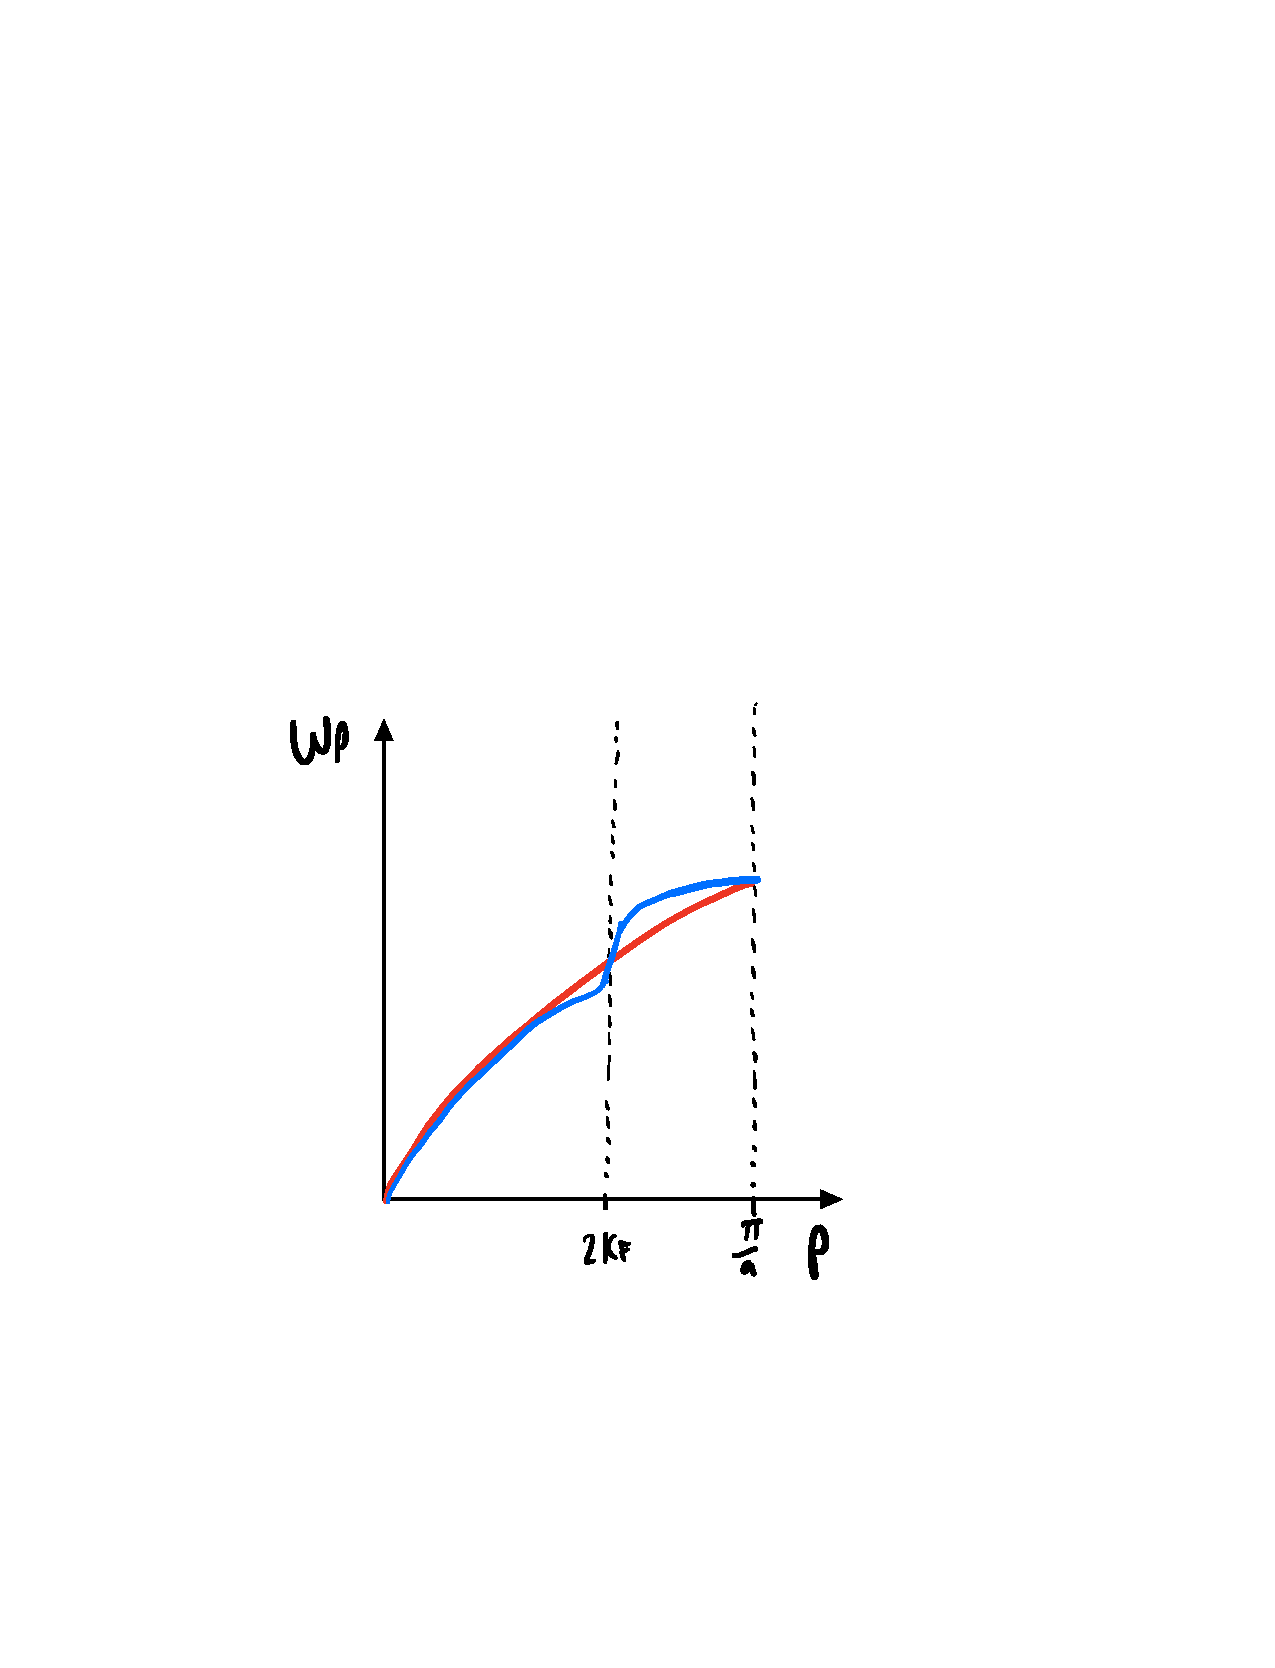
\includegraphics[scale=0.6]{Images/fig-kohndispersion.pdf}
    \caption{Dispersion Relation for 3-D electron-phonon interaction Hamiltonian. The derivative of the dispersion diverges at $p = 2k_F$.}
    \label{fig-kohndispersion}
\end{figure}

What's the intuition behind this? Diagramatically, we have a electron-hole bubble:

\begin{figure}[htbp]
    \centering
    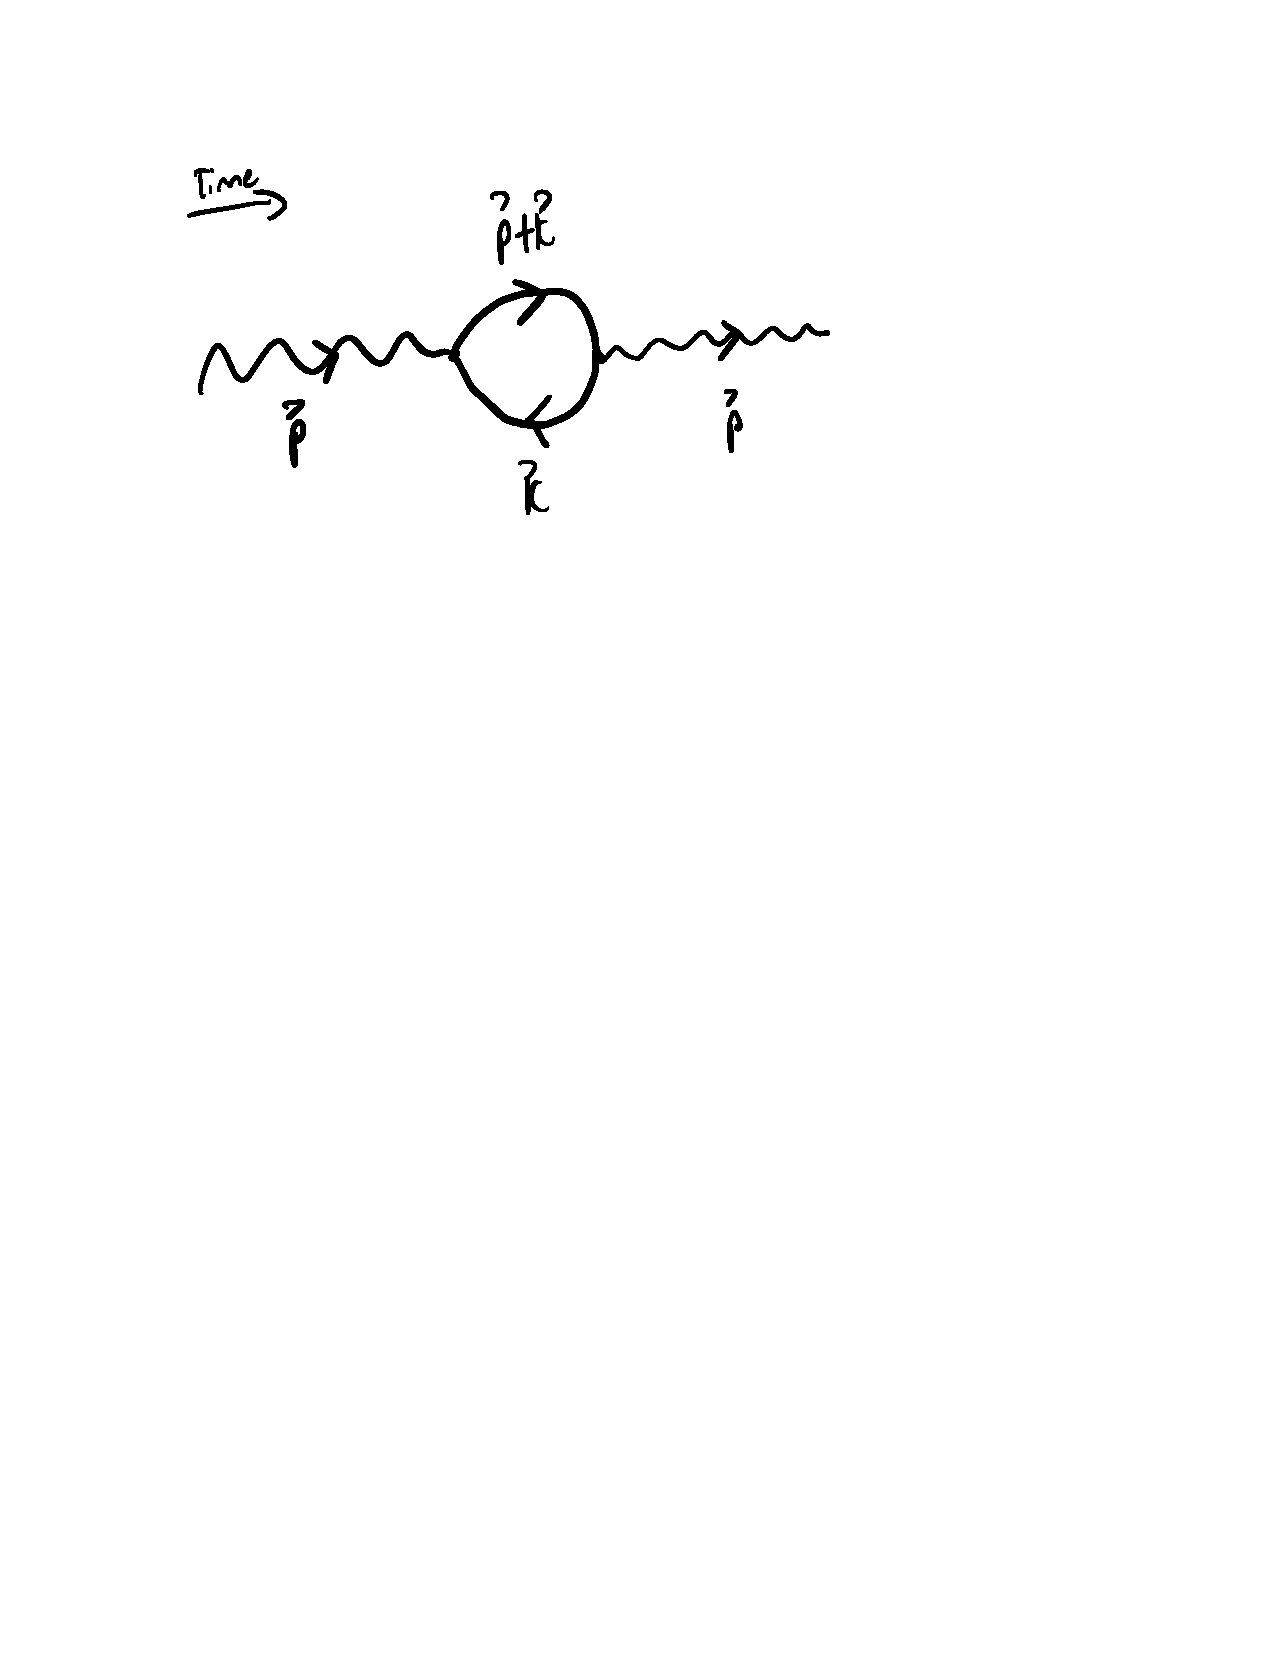
\includegraphics[scale=0.8]{Images/fig-electronholebubble.pdf}
    \caption{Feynman Diagram of Electron-Hole Bubble.}
    \label{fig-electronholebubble}
\end{figure}

and why does this give us the intuition for the anomaly? Intuitively, the Kohn anomaly can be interpreted as phonon spending some fraction of time as a electron-hole pair. Because $v_F \gg v_{ph}$, the phonon speed of propagation increases dramatically. Why only near the fermi momentum? Kinetmatic constraints - you need the correct amount of momentum to create an electron-hole pair. At precisely $2k_F$, the fraction of time the phonon spends as an electron-hole pair approaches 100\%. Note a more careful analysis of the behaviour near $2k_F$ would show that the derivative of the dispersion does not actually diverge but approaches the fermi velocity, as we might expect.

\subsubsection{1 dimension - Peirels Instability}
Assume $\abs{\omega_q} \ll \e_k, \e_{k+p}$. We then evaluate:
\begin{equation}
    \hbar \delta \omega_p = -\int_{-\infty}^\infty dk \frac{n_k(1 - n_{k-q})}{\e_{k - q} - \e_k}
\end{equation}
but the integral vanishes everywhere where the product of $n_k, (1 - n_{k-q})$ is not supported, i.e. everywhere except $[-k_F, -k_F + q]$ (see sketch below)

\begin{figure}[htbp]
    \centering
    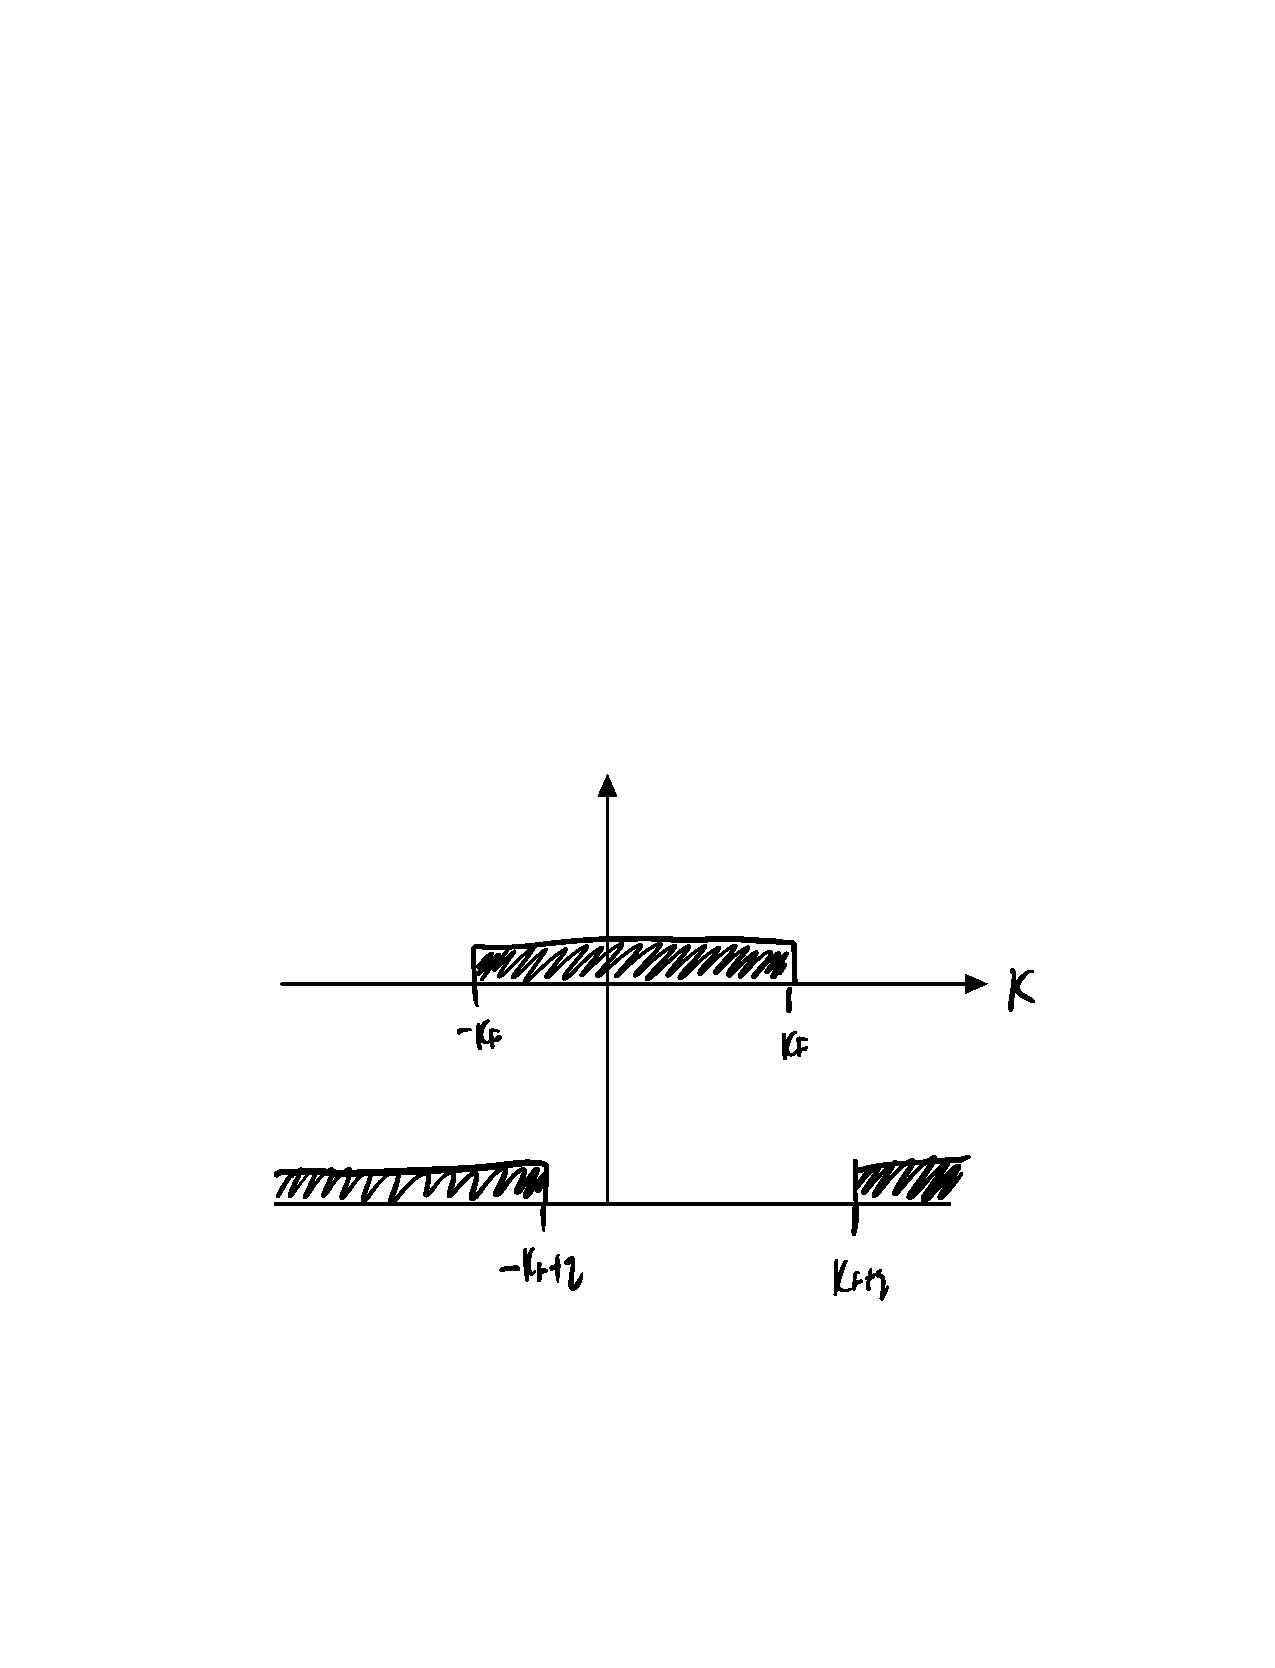
\includegraphics[scale=0.6]{Images/fig-peirelssupport.pdf}
    \caption{Sketch of the support of $n_k, 1 - n_{k-q}$.}
    \label{fig-peirelssupport}
\end{figure}

so:
\begin{equation}
    \hbar \delta \omega_P =  -\int_{-k_F}^{-k_F + q}dk \frac{1}{(k - q)^2 - k^2} = \left.\frac{1}{2q}\ln\abs{q - 2k}\right|_{-k_F}^{q - k_F} = \frac{1}{2q}\left(\ln\abs{q - 2k_F} - \ln\abs{q + 2k_F}\right)
\end{equation}
Although we assume $q > 0$, the same occurs for $q < 0$, as the above is symmetric in the sign of $q$. But now notice - this correction is divergent when $q = \pm 2k_F$! This is a much stronger effect - in 3D the correction was finite but the derivative diverged, but here the correction itself diverges.

\begin{figure}[htbp]
    \centering
    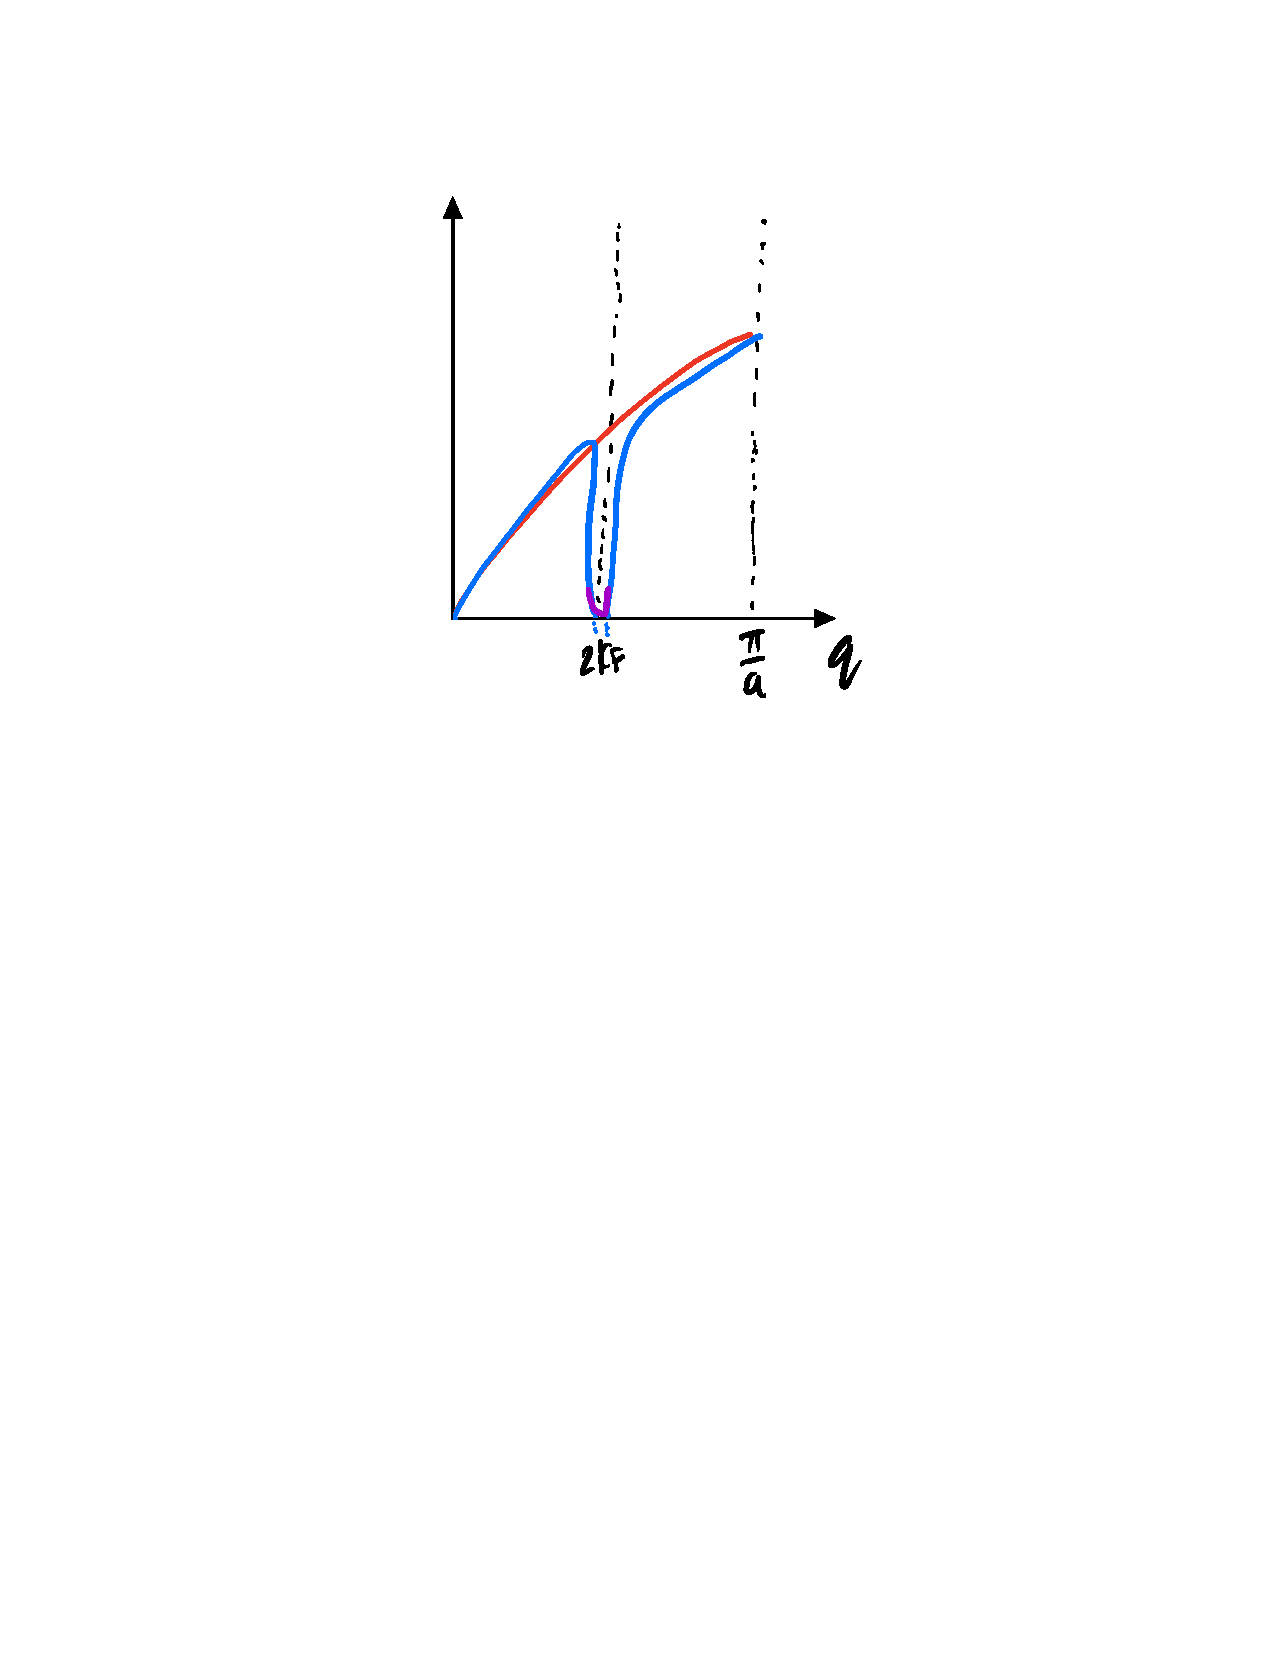
\includegraphics[scale=0.7]{Images/fig-peirelsdispersion.pdf}
    \caption{Dispersion Relation for 1-D electron-phonon interaction Hamiltonian. Naive analysis has the dispersion (blue) diverging at $q = 2k_F$ but otherwise similar to the original dispersion (red), but a more careful analysis shows that the dispersion goes to zero at $2k_F$ instead (purple).}
    \label{fig-peirelsdispersion}
\end{figure}

Note: A more careful treatement where we do not neglect $\hbar \omega_q$ in the denominator shows that $\omega_q \to 0$ as $q \to 2k_F$ (rather than diverging). This leads to ``Bose Condensation'' of phonons at $q = \pm 2k_F$ - there is always a macroscopic number of phonons at this frequency, as there is no energy cost to be at that frequency. Physically, what does this mean? This corresponds to a static distortion of the lattice (we see a spontaneous change in the geometry), known as the \emph{Peierls instability}. Next time we look at the canonical example of this, which is polyacetate - it undergoes a dimerization transition which can be observed as this instability.